\documentclass{beamer}
\usepackage{geometry}
\usepackage[english]{babel}
\usepackage[utf8]{inputenc}
\usepackage{amsmath}
\usepackage{amsfonts}
\usepackage{amssymb}
\usepackage{tikz}
\usepackage{graphicx}
\usepackage{venndiagram}

%\usepackage{pgfplots}
%\pgfplotsset{width=10cm,compat=1.9}
%\usepackage{pgfplotstable}

\setlength{\headheight}{26pt}%doesn't seem to fix warning

\usepackage{fancyhdr}
\pagestyle{fancy}
\fancyhf{}

%\rhead{\small{21 May 2018}}
\lhead{\small{BECA / Dr. Huson / Mathematics}}

%\vspace{1cm}

\renewcommand{\headrulewidth}{0pt}


\title{Mathematics Class Slides}
\subtitle{Bronx Early College Academy}
\author{Chris Huson}
\date{27 August [was 23 May] 2018}

\begin{document}

\frame{\titlepage}

%\section[Outline]{}
%\frame{\tableofcontents}


\section{11.2 Drui}
\frame
{
  \frametitle{GQ: How do we organize data using frequency distributions?}
  \framesubtitle{CCSS: HSS.CP.B.6 Probabilities \qquad \qquad \qquad \alert{11.2}}

  \begin{block}{Do Now: Write the formula and perform the calculation}
  \begin{enumerate}
      \item How many groups of 2 students may be selected from a class of 12?
      \item How many groups of 10 students may be selected from a class of 12?
  \end{enumerate}
  \end{block}
  Lesson: Subsets, frequency distributions\\*[5pt]
  Task: Combinatorics problem\\*[5pt]
  Assessment: Final homework problem\\*[5pt]
  Homework: Set theory handout
}

\section{11.2 Drui}
\frame
{
  \frametitle{GQ: How do we graph polynomials?}
  \framesubtitle{CCSS: HSS.CP.B.6 Understand polynomial functions \qquad \qquad \qquad \alert{11.2}}

  \begin{block}{Do Now: Write down vocabulary words in notebook}
  \begin{enumerate}
    \item Standard form, factored form, order, degree\\*[5pt]
    \item substitution, long division, remainder\\*[5pt]
    \item $x$-intercepts, zeros, roots, solutions\\*[5pt]
    \item $y$-intercept\\*[5pt]
    \item end behavior, increasing/decreasing, turning points\\*[5pt]
    \item symmetry, odd/even\\*[5pt]
  \end{enumerate}
  \end{block}
  Lesson: Features of polynomial functions p. 280\\*[5pt]
  Task: Problems \# 8-19 odds, 32-37 p. 285\\*[5pt]
  Assessment: Graphing\\*[5pt]
  Homework: Workbook p. 119
}

\frame
{
  \frametitle{Graphing polynomials}
  \framesubtitle{Evaluating functions using the distributive property and substitution \qquad \qquad \qquad \alert{11.2}}

  \begin{block}{Group presentations}
  \begin{enumerate}
      \item $f(x)=x^3-5x^2+2x+8$ \qquad Group A\\*[10pt]
      %$f(x)=(x-2)(x-4)(x+1)$\\*
      \item $g(x)=-x^3-7x^2-14x-8$ \qquad Group B\\*[10pt]
      %$g(x)=(x-2)(x-4)(x+1)$\\*
      \item $h(x)=-x^3-4x$ \qquad \qquad \qquad Group C\\*[10pt]
      \item $j(x)=x^3+2x^2-5x-6$ \qquad Group D\\*[10pt]
      \item $k(x)=-x^3+4x$\\*
      $k(x)=-x(x+2)(x-2)$ \qquad Group D\\*[10pt]

  \end{enumerate}
  \end{block}
}
\frame
{
  \frametitle{Graphing polynomials}
  \framesubtitle{Evaluating functions using the distributive property and substitution \qquad \qquad \qquad \alert{11.2}}

  \begin{block}{Do Now: }
  \begin{enumerate}
      \item Group A:       $f\left(x\right)=x^3+2x^2-5x-6$
      $g\left(x\right)=\left(x-2\right)\left(x-4\right)\left(x+1\right)$\\*

  \end{enumerate}
  \end{block}
}

\frame
{
  \frametitle{Polynomials}
  \framesubtitle{Each polynomial function can be shown in two forms: standard and factored. \qquad \qquad \qquad \alert{11.2}}
\alert{Standard form}: From largest exponent to smallest\\*
\qquad \alert{Order or degree}: value of the largest exponent\\*
\qquad \alert{Constant term}: the ones value (8, in the example below)
\alert{Factored form}: Product of binomials\\*
\qquad \alert{Factor}: each monomial (e.g. "$(x+1)$)\\*[15pt]
  \begin{enumerate}
    \item Evaluate $f(0)$ and $f(2)$ for each function below.
      \item $f(x)=x^3-5x^2+2x+8$ \qquad \\*[10pt]
      $f(x)=(x+1)(x-2)(x-4)$\\*

  \end{enumerate}
}

\begin{frame}{Vocabulary for polynomial functions}
    Standard form, factored form, order, degree\\*[5pt]
    substitution, long division, remainder\\*[5pt]
    $x$-intercepts, zeros, roots, solutions\\*[5pt]
    $y$-intercept\\*[5pt]
    end behavior, increasing/decreasing, turning points\\*[5pt]
    symmetry, odd/even\\*[5pt]
\end{frame}

\section{11.2 Algebra II Drui}
\frame
{
  \frametitle{How do we convert the base of an exponential function?}
  \framesubtitle{CCSS: HSF.LB.B.5 Interpret the parameters in an exponential function in context \qquad \alert{11.2}}

  \begin{block}{Do Now: Exponent practice. Simplify:}
  \begin{enumerate}
      \item $a^3 \times b^2 \times a^2$
      \item $x^3 \cdot y^2 \div x^3$
      \item $\displaystyle m^\frac{1}{3} \times m^\frac{4}{3} \times m^\frac{1}{3}$
      \item $z^4 \cdot z^{-1} \cdot z^{-2}$
  \end{enumerate}
  \end{block}
  Lesson: Consolidating a coefficient into the base of an exponential\\*
  Task: Practice problems\\*
  Assessment: Test corrections due today\\*
  Homework: Exponential function \& review problems\\
}


\section{11.2 Algebra II Drui}
\frame
{
  \frametitle{How do we convert the base of an exponential function?}
  \framesubtitle{CCSS: HSF.LB.B.5 Interpret the parameters in an exponential function \qquad \alert{11.2}}

  \begin{block}{Do Now: Interest calculations, assume principal is \$100.}
  \begin{enumerate}
      \item Calculate interest for 6 months with an annual rate of 5\%.
      \item After one year at an annual rate of 5.25\%, what would be the combined principal and interest?
      \item How many interest payments would there be in two years given monthly compounding?
      \item If the interest after one month is \$1.50, what would the annual interest rate be?
  \end{enumerate}
  \end{block}
  Lesson: Continuously compounded interest\\*
  Task: Practice problems\\*
  Assessment: Convert to an annual rate given $P=P_0e^{0.05x}$\\*
  Homework: Exponential function \& review problems\\
}


\section{11.2 Algebra II Drui}
\frame
{
  \frametitle{How do we convert the base of an exponential function?}
  \framesubtitle{CCSS: HSF.LB.B.5 Interpret the parameters in an exponential function \qquad \alert{11.2}}

  \begin{block}{Do Now: An investment of \$1,500 earns a continuous interest rate of 2.25\%. }
  \begin{enumerate}
      \item Write down the value of the investment as a function of time in years: $f(t)=$
      \item How much would the investment be worth after 10 years? How much of that is interest?
      \item Use a graphing calculator to compare two functions: $y=1500 \times e^{(10x)}$ and $y=3000$.
      \item For what $x$ are the functions equal? What does this point represent?
  \end{enumerate}
  \end{block}
  Lesson: Homework problem set review, exponential functions\\*
  Task: Graphing and function problems\\*
  Assessment: \alert{Exam Thursday}\\
  Homework: Pretest problem set\\
}

\section{11.2 Algebra II Drui}
\frame
{
  \frametitle{How do we convert the base of an exponential function?}
  \framesubtitle{CCSS: HSF.LB.B.5 Interpret the parameters in an exponential function \qquad \alert{11.2}}

  \begin{block}{Do Now: Exam review problems}
  \begin{enumerate}
    \item Evaluate $f(x)=\sqrt{x^2}$ for $x=-2, -1, 0, 1, 2$
    \item Sketch the function for $x \in \mathbb{R}$.
    \item Write down another representation of $f(x)$.
    \item Solve for $a$ where $a^x=(e^{0.03925})^x$
    \end{enumerate}
  \end{block}
  Lesson: Exam results, substituting into formulas, precision\\*
  Homework: Test corrections due tomorrow\\}

\section{11.2 Algebra II Drui}
\frame
{
  \frametitle{How do we use and interpret trigonometric functions?}
  \framesubtitle{HSF.LB.B.5 Interpret the parameters in a trigonometric function in context \qquad \alert{11.2}}

  \begin{block}{Do Now: Exam review problems}
  \begin{enumerate}
    \item Handout practice of graphing and solving%Evaluate $f(x)=\sqrt{x^2}$ for $x=-2, -1, 0, 1, 2$
    %\item Sketch the function for $x \in \mathbb{R}$.
    %\item Write down another representation of $f(x)$.
    %\item Solve for $a$ where $a^x=(e^{0.03925})^x$
    \end{enumerate}
  \end{block}
  Lesson: Using periodic functions for modeling\\*
  Task: Regents practice - Complete mastery grid cells\\*
  Assessment: Test \alert{tomorrow}\\*
  Homework: Study pretest problems for test\\}
  
  \section{12.1 Drui}
  \frame
  {
    \frametitle{GQ: How do we calculate area with integration?}
    \framesubtitle{CCSS: F.IF.B.6 Calculate \& interpret the rate of change of a function}

    \begin{block}{Do Now}
    \begin{enumerate}
        \item Find $\int{(4x^3-3x+1)}\mathrm{d}x$.
        \item Find $\int e^{5x}\mathrm{d}x$.
        \item Find $\displaystyle \int \frac{1}{3x+1} \mathrm{d}x$.
    \end{enumerate}
    Homework review \#1, 5, 6 p. 302
    \end{block}
    Lesson: Reimann sums and the definite integral\\*[5pt]
    Task: Example 8, page 304\\*[5pt]
    Assessment: Calculator integration \\*[5pt]
    Homework: Exercises 9H evens p. 308
  }

  \section{12.1 Drui}
  \frame
  {
    \frametitle{GQ: How do we calculate area with definite integrals?}
    \framesubtitle{CCSS: F.IF.B.6 Calculate \& interpret the rate of change of a function}

    \begin{block}{Do Now}
    \begin{enumerate}
        \item Use a calculator to find $\displaystyle \int_0^{\frac{\pi}{2}}{\cos x}\ \mathrm{d}x$
        \item Differentiate $y=\sqrt{3x^3-x}$
        \item Find $\int{(6x^2-2x-5)}\mathrm{d}x$.
        \item Differentiate $y={(3x^2-5x)^5}$
        \item Find $\int 5(x^2+1)^4(2x)\mathrm{d}x$.
        \item Find $\displaystyle \int \frac{3}{x}\ \mathrm{d}x$.
    \end{enumerate}
    \end{block}
    Lesson: Properties of definite integrals p. 307\\%*[5pt]
    Task: Review homework problems\\%*[5pt]
    Assessment: Problem \#11 p. 300 \\%*[5pt]
    Homework: Exercises 9H evens p. 308
  }

  \section{12.1 Drui}
  \frame
  {
    \frametitle{GQ: How do we calculate area with definite integrals?}
    \framesubtitle{CCSS: F.IF.B.6 Calculate \& interpret the rate of change of a function}

    \begin{block}{Do Now}
    \begin{enumerate}
        \item Use a calculator to find $\displaystyle \int_{-1}^{1}{\frac{1}{x+2}}\ \mathrm{d}x$
        \item Differentiate $y=\sqrt[3]{5x^2-2x}$
        \item Find $\int{(6x^2-2)^4(12x)} \ \mathrm{d}x$.
        \item Differentiate $y={(3x^2-5x)(\ln x)}$
        \item Find $\displaystyle \int_1^2 \frac{3}{x^2}\ \mathrm{d}x$. (check your result with a calculator)
    \end{enumerate}
    \end{block}
    Lesson: The fundamental theorem of calculus p. 309\\%*[5pt]
    Task: Practice Examples 11, 12 p. 310-1\\%*[5pt]
    Assessment: Problem 9J \#1 p. 312 \\%*[5pt]
    Homework: Exercises 9I, 9J p. 310-12
  }

  \section{12.1 Drui}
  \frame
  {
    \frametitle{GQ: How do we calculate the area between two curves?}
    \framesubtitle{CCSS: F.IF.B.6 Calculate \& interpret the rate of change of a function}

    \begin{block}{Do Now: Consider the function $f(x)=-x^2+2x+3$}
    \begin{enumerate}
        \item Factor $f$ and state its zeros.
        \item Restate $f$ in vertex form. Write down the vertex as an ordered pair.
        \item Differentiate $f$. Show that the zero of $f^\prime(x)$ is the vertex of $f$.
        \item If $f(x)$ represents the height of a diver over the domain $0 \leq x \leq 3$, interpret $f(0)$ and $f^\prime(0)$
        \item What is the size of the area bounded by $f$, $x=0$, and $y=0$?
    \end{enumerate}
    \end{block}
    Lesson: The area between two functions p. 313\\%*[5pt]
    %Task: Practice Examples 11, 12 p. 310-1\\%*[5pt]
    Assessment: Example \#13 p. 314 \\%*[5pt]
    Homework: Exercises 9K p. 316
  }

  \section{12.1 Drui}
  \frame
  {
    \frametitle{GQ: How do we calculate a volume of rotation?}
    \framesubtitle{CCSS: F.IF.B.6 Calculate \& interpret the rate of change of a function}

    \begin{block}{Do Now: Sketch the functions $f(x)=10x+x^2-3x^3$ and $g(x)=x^2-2x$}
    \begin{enumerate}
        \item What are their intersections? (i.e. $f(x)=g(x)$)
        \item What is the definite integral representing the area between the curves?
        \item Using a calculator, what is the size of the area? (this may not be a trivial question)
    \end{enumerate}
    \end{block}
    Lesson: Integrating circle areas, modeling a solid p. 318\\%*[5pt]
    %Task: Practice Examples 11, 12 p. 310-1\\%*[5pt]
    Assessment: Example \#15 p. 319 \\%*[5pt]
    Homework: Exercises 9L \& 9M p. 317, 319; probability handout
  }

  \section{12.1 Drui}
  \frame
  {
    \frametitle{GQ: How do we calculate displacement from velocity?}
    \framesubtitle{CCSS: F.IF.B.6 Calculate \& interpret the rate of change of a function \qquad \alert{12.1}}

    \begin{block}{Do Now: Do the calculations below and read the handout}
    \begin{enumerate}
        \item Lance Armstrong’s average speed in his six Tour de France victories from 1999-2004 was about 24 miles per hour. Assuming that he pedals at his average speed and takes no breaks, how long would it take him to ride 38 miles to the top of a 10,000 ft. volcano?
        \item People who are not Lance Armstrong can travel at about 12 miles per hour on a bike. At that speed, how long would it take to reach the top of the volcano?
    \end{enumerate}
    \end{block}
    Lesson: Integrating velocity over time, displacement p. 321\\%*[5pt]
    %Task: Practice Examples 11, 12 p. 310-1\\%*[5pt]
    Assessment: Example \#18 p. 323 \\%*[5pt]
    Homework: Exercises 9N \& 9O p. 320, 324
  }

  \section{12.1 Drui}
  \frame
  {
    \frametitle{GQ: How do we calculate displacement from velocity?}
    \framesubtitle{CCSS: F.IF.B.6 Calculate \& interpret the rate of change of a function \qquad \alert{12.1}}

    \begin{block}{Do Now: continued, 38 mile ride in 10 hours}
    \begin{enumerate}
        \item Using the velocity vs time graph from yesterday, integrate to show that the areas representing the distance covered by the three riders are equal ($v \times t = d$).
        \item Show that a rider accelerating according to $v(t)= \frac{76}{100}t$ also arrives at $(10,38)$.
    \end{enumerate}
    \end{block}
    Lesson: Integrating velocity over time, displacement p. 321\\%*[5pt]
    Task: Review 9F, 9M, probability\\%*[5pt]
    Assessment: Example \#18 p. 323 (take home test Thursday)\\%*[5pt]
    Homework: Exercises 9P p. 326, any remaining problem sets
  }

  \section{12.1 Drui}
  \frame
  {
    \frametitle{GQ: How does a function's graph relate to its derivatives?}
    \framesubtitle{CCSS: HSF.IF.B.4 Interpret key features of functions and their graphs \qquad \alert{12.1}}

    \begin{block}{Do Now: Differential calculus}
    \begin{enumerate}
        \item Take the 1st \& 2nd derivatives of $f(x)=x^3-6x^2+6x$.
        \item Sketch the function.\\*
        Challenge: Identify key features, graphically \& algebraically.
    \end{enumerate}
    \end{block}
    Lesson: Function graphs, extrema, the 1st \& 2nd derivative tests p. 233, 240\\%*[5pt]
    Task: 7Q p. 232 \#1-3; 7R p. 234 1, 2; 7S p. 236 1, 3 \\%*[5pt]
    Assessment: Handout graphing problem \#1 (\#2 challenge)
    \\%*[5pt]
    Homework: IB function / graphing problem set
  }

  \section{12.1 Drui}
  \frame
  {
    \frametitle{GQ: How does a function's graph relate to its derivatives?}
    \framesubtitle{CCSS: HSF.IF.B.4 Interpret key features of functions and their graphs \qquad \alert{12.1}}

    \begin{block}{Do Now: Given $f(x)=x \cos x, 0 \leq x \leq 2\pi$.}
    \begin{enumerate}
        \item Take the 1st \& 2nd derivatives of $f(x)$. \item Sketch the function. \item Over what intervals is the function increasing, decreasing?
    \end{enumerate}
    \end{block}
    Lesson: Function graphs, extrema, the 1st \& 2nd derivative tests p. 233, 240\\%*[5pt]
    Task: 7Q p. 232 \#1-3; 7R p. 234 1, 2; 7S p. 236 1, 3 \\%*[5pt]
    Assessment: Handout graphing problem \#1 (\#2 challenge)
    \\%*[5pt]
    Homework: Test corrections Paper 1
  }

  \section{12.1 Drui}
  \frame
  {
    \frametitle{GQ: How does a function's graph relate to its derivatives?}
    \framesubtitle{CCSS: HSF.IF.B.4 Interpret key features of functions and their graphs \qquad \alert{12.1}}

    \begin{block}{Do Now: Given $f\left(x\right) =-x^4 +2x^2 +x$. There are $x$-intercepts at $x=0$ and $x=p$. There is a maximum at A where $x=a$, and a point of inflection at B where $x=b$.}
    \begin{enumerate}
        \item Find the value of $p$.
        \item Write down the coordinates of A.
        \item Write down the rate of change of $f$ at A.
        \item Find the coordinates of B.
        \item Write down the rate of change of $f$ at B.
    \end{enumerate}
    \end{block}
    Lesson: The 1st \& 2nd derivative tests p. 233, 240\\%*[5pt]
    Task: 7Q p. 232 \#1-3; 7R p. 234 1, 2; 7S p. 236 1, 3 \\%*[5pt]
    Assessment: Calculator calculus functions in Do Now.
    \\%*[5pt]
    Homework: Handout IB function / graphing problem set
  }

  \section{12.1 Drui}
  \frame
  {
    \frametitle{GQ: How does a function's graph relate to its derivatives?}
    \framesubtitle{CCSS: HSF.IF.B.4 Interpret key features of functions and their graphs \qquad \alert{12.1}}

    \begin{block}{Do Now: Find the 1st derivative of the function and solve for it's zeros as potential extrema (stationary points). Use the 1st derivative test to determine whether it is a max, min, or neither.}
    \begin{enumerate}
        \item $f(x)=x^3$.
        \item $\displaystyle f(x)=\frac{x^2-4}{x^2-1}$
    \end{enumerate}
    \end{block}
    Lesson: The 1st \& 2nd derivative tests p. 233, 240\\%*[5pt]
    Task: Homework review; 7Q p. 232 \#1-3; 7R p. 234 1, 2; 7S p. 236 1, 3 \\%*[5pt]
    Assessment: Use of the 1st \& 2nd derivative tests
    \\%*[5pt]
    Homework: Study for test \alert{tomorrow}
  }

  \section{12.1 Drui}
  \frame
  {
    \frametitle{GQ: How is the binomial expansion like a probability tree?}
    \framesubtitle{CCSS: HSS.MD.A.3 Develop a probability distribution for a random variable \qquad \alert{12.1}}

    \begin{block}{Do Now: Make a tree representing three coin flips}
    \begin{enumerate}
        \item What is the probability of each outcome?
        \item If order doesn't matter, how can the results be consolidated into a probability distribution of the total number of heads?
    \end{enumerate}
    \end{block}
    Lesson:  Binomial expansion p. 186-8\\%*[5pt]
    Task: IB exam paper problems\\%*[5pt]
    Assessment: Test corrections due Thursday (snow pending)
    \\%*[5pt]
    Homework: Complete probability problem set
  }

  \section{12.1 Drui}
  \frame
  {
    \frametitle{GQ: How do we summarize the features of a population?}
    \framesubtitle{CCSS: HSS.MD.A.3 Develop a probability distribution for a random variable \qquad \alert{12.1}}

    \begin{block}{Do Now: Given $f(x)=x^2+3x$. \\*
    (work on paper you can turn in.}
    \begin{enumerate}
        \item Find $f'(x)$.
        \item What is the equation of the tangent to $f$ at $x=1$?
        \item Plot both $f$ and the tangent on your graphing calculator.
    \end{enumerate}
    \end{block}
    Lesson:  Cumulative distributions, summative stats p. 42-72\\%*[5pt]
    Task: Grouped frequency table calculations\\%*[5pt]
    Assessment: Problem \#3 2H p. 60
    \\%*[5pt]
    Homework: Problem set, univariate data statistics
  }


  \section{12.1 Drui}
  \frame
  {
    \frametitle{GQ: How do we interpret a cumulative distribution graph?}
    \framesubtitle{CCSS: HSS.MD.A.3 Develop a probability distribution for a random variable \qquad \alert{12.1}}

    \begin{block}{Do Now: Given the data in problem \#3 2H p. 60.\\*
    (work on paper you can turn in.)}
      \begin{enumerate}
        \item Write down the modal class.
        \item Write a formula for the mean test result.
        \item Compute the mean using the calculator stats function.
      \end{enumerate}
   \end{block}
    Homework review\\*
    Lesson:  Dispersion p. 73-83, Normal distributions p. 204-216\\%*[5pt]
    Task: Problem \#1 2K p. 72\\%*[5pt]
    Assessment: Problem \#7 Review exercise p. 79
    \\%*[5pt]
    Homework: Problem set, cumulative distributions
  }



  \section{12.1 Drui}
  \frame
  {
    \frametitle{GQ: How do we use the normal curve?}
    \framesubtitle{CCSS: HSS.MD.A.3 Develop a probability distribution for a random variable \qquad \alert{12.1}}

    \begin{block}{Do Now}
      \begin{enumerate}
      \item Confirm the regression equation fit to \#4 p. 348.
      \item How would you interpret the correlation of two variables having $r=-0.65$? (p. 359)
      \item Sketch a normal curve with $X\sim N(500, 100^2)$.
      \href{https://blog.prepscholar.com/sat-standard-deviation}{link}
      \end{enumerate}
   \end{block}
    Homework review\\*
    Lesson:  Regression, residuals, least-squares, extrapolation, mean point $(\bar{x},\bar{y})$ (p. 334-359)\\*
    Normal distribution, Z-score, inverse normal (p. 538-553) \\%*[5pt]
    Task: The standard normal and Z-score problems, 15H p. 541\\%*[5pt]
    Assessment: Exercise 15H \#1 \& 5 p. 541\\%*[5pt]
    Homework: Problem set regressions, probability distributions
  }

  \section{12.1 Drui}
  \frame
  {
    \frametitle{GQ: How do we use the inverse normal function?}
    \framesubtitle{CCSS: HSS.MD.A.3 Develop a probability distribution for a random variable \qquad \alert{12.1}}

    \begin{block}{Do Now: What formulas applying to pretest problems 4c \& 4d?}
      \begin{enumerate}
      \item Given $A$ and $B$ are independent and $\mathrm{P}(A)=0.2$, $\mathrm{P}(B)=0.8$. Find $\mathrm{P}(A \cap B)$
      \item \href{https://blog.prepscholar.com/sat-standard-deviation}{SAT link}
      \end{enumerate}
   \end{block}
    Pretest packet homework review\\*
    Lesson: Chapter 15 summary p. 553\\%*[5pt]
    Task: Review exercises p. 551\\%*[5pt]
    Assessment: Exam this week\\%*[5pt]
    Homework: IB problem set
  }


  \section{12.1 Drui}
  \frame
  {
    \frametitle{GQ: How do we integrate a function?}
    \framesubtitle{CCSS: HSF.IF.B.6 Calculate and interpret the area under a function \qquad \alert{12.1}}

    \begin{block}{Do Now: Chain rule - Take the derivative of each function}
      \begin{enumerate}
      \item $f(x)=\sin{x^3}$
      \item $g(x)=\sqrt{x^4+2}$
      \item $h(x)=\ln{(x^2+1)}$
      \end{enumerate}
   \end{block}
    Lesson: Take home exam papers assessment \& review\\%*[5pt]
    Task: Work problems on board\\%*[5pt]
    Assessment: Test corrections due\\%*[5pt]
    Homework: Integration exam problems
  }

  \section{12.1 Drui}
  \frame
  {
    \frametitle{GQ: How do we calculate volume (of a rotated function)?}
    \framesubtitle{CCSS: HSF.IF.B.6 Calculate and interpret the area under a function \qquad \alert{12.1}}

    \begin{block}{Do Now: Identifying problem types. On your homework, underline the ``M1" points you earned. Examples:}
      \begin{enumerate}
      \item $X \sim B(10, 0.5)$
      \item bell curve sketch
      \item $u= \& \quad u'=$
      \end{enumerate}
   \end{block}
    Lesson: $\displaystyle \int_a^b \pi r^2 \text{d}x$\\%*[5pt]
    Task: Work homework problems on board\\%*[5pt]
    Assessment: self-reflection on mixed versus block problem sets\\%*[5pt]
    Homework: Solids of rotation \& mixed exam problems
  }


  \section{12.1 Drui}
  \frame
  {
    \frametitle{GQ: How do we use periodic functions?}
    \framesubtitle{CCSS: HSF.TF.A.3 Extend trig functions with the unit circle \qquad \alert{12.1}}

    \begin{block}{Do Now: Create a unit circle and label the standard angles with their coordinate pairs.}
      %\begin{enumerate}
      %\item $\displaystyle \int_a^b \pi f^2 %\text{d}x$
      %\item ``$u$" substitution: $u= \& \quad u'=$
      %\end{enumerate}
   \end{block}
    Homework review, particularly: \\ $\displaystyle \int_a^b \pi f^2 \text{d}x$ \&
  ``$u$" substitution: $u= \& \quad u'=$\\[5pt]
    Lesson: Periodic functions\\%*[5pt]
    Task: Work homework problems on board\\%*[5pt]
    Assessment: problem set mark scheme\\%*[5pt]
    Homework: Sine curves \& mixed exam problems
  }


  \section{12.1 Drui}
  \frame
  {
    \frametitle{GQ: How do we use periodic functions?}
    \framesubtitle{CCSS: HSF.TF.A.3 Extend trig functions with the unit circle \qquad \alert{12.1}}

    \begin{block}{Do Now: Sketch the periodic function $f(x)=\sin{x}$}
      \begin{enumerate}
      \item Label the $x$-axis with multiples of $\pi$, including standard fractions in the first quadrant
      \item Mark the $y$-axis with the values of the standard angles (positive and negative).
      \item Mark points on the curve at the standard angles.
      \end{enumerate}
   \end{block}
    Homework review\\[5pt]
    Lesson: Applications calculating the period as $\frac{2\pi}{b}$\\%*[5pt]
    Task: Work homework problems on board\\%*[5pt]
    Assessment: problem set mark scheme\\%*[5pt]
    Homework: Trig \& mixed exam problems
  }

  \section{12.1 IB Math SL Drui}
  \frame
  {
    \frametitle{GQ: How do we use periodic functions?}
    \framesubtitle{CCSS: HSF.TF.A.3 Extend trig functions with the unit circle \qquad \alert{12.1}}

    \begin{block}{Do Now: Refresh your trigonometry!}
      \begin{enumerate}
      \item Sketch the periodic functions $f(x)=\sin{x}$ and $g(x)=\cos{x}$ on the same axes
      \item Draw the unit circle, marking the standard angles and noting their trig values: $(x=\cos{\theta}, y=\sin{\theta})$.
      \item Identify the parameters of $y=a\sin{(bx-h)}+k$
      \item In your calculator graph $f(x)=\tan{x}$
      \end{enumerate}
   \end{block}
    Lesson: Homework review\\[5pt]
    Task: Work homework problems on board\\%*[5pt]
    Assessment: problem set mark scheme\\%*[5pt]
    Homework: Trig \& mixed exam problems
  }

  \section{12.1 IB Math SL Drui}
  \frame
  {
    \frametitle{GQ: How do we prepare for the IB final exams?}
    \framesubtitle{CCSS: HSF.IF.B.4 Interpret key features of functions and their graphs \qquad \alert{12.1}}

    \begin{block}{Do Now: 1st \& 2nd derivatives of a cubic function, sketch}
      \begin{enumerate}
      \item Given the function $f(x)=x^3-9x$
      \item Find $f'(x)$ and $f''(x)$.
      \item Sketch $f$ and its two derivatives on the same set of axes. Label the intersections and extrema.
      \end{enumerate}
   \end{block}
    Lesson: Last minute study practices (reflection) \\[5pt]
    Task: Homework review: Work homework problems on board\\%*[5pt]
    Assessment: Problem set and exam mark scheme\\%*[5pt]
    Homework: Prepare for final exams
  }

  \frame
  {
    \frametitle{The volume of a function rotated around the $x$-axis}
    \framesubtitle{Differentiate over $x$, but use the area of a disk defined by $A=\pi r^2$}
  \href{https://www.youtube.com/watch?v=i4L5XoUBD_Q}{video}\\
  \begin{figure}[!ht]
      \centering
      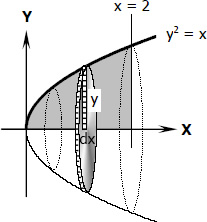
\includegraphics[width=0.5\textwidth]{0413CW-paraboloid.jpg}
  \end{figure}
  \small{Credit: MATHalino.com - Pinoy Math Community Romel Verterra}
  }

  \frame
  {
    \frametitle{Interpreting a displacement vs time graph}
    \framesubtitle{CCSS: F.IF.B.6 Calculate \& interpret the rate of change of a function}

    \begin{block}{Consider the function $f(x)=-x^2+2x+3$}
    \begin{enumerate}
        \item Factor $f$ and state its zeros.
        \item Restate $f$ in vertex form. Write down the vertex as an ordered pair.
        \item Over what intervals is the function increasing, decreasing, and neither?
        \item If $f(x)$ represents the height of a diver over the domain $0 \leq x \leq 3$, interpret $f(0)$, the vertex, and $f(3)$
        \item What does the "slope" of the curve represent?
    \end{enumerate}
    \end{block}
  }

  \section{12.1 IB Math SL Drui}
  \frame
  {
    \frametitle{GQ: How do we prepare for the IB final exams?}
    \framesubtitle{CCSS: HSF.IF.B.4 Interpret key features of functions and their graphs \qquad \alert{12.1}}

    \begin{block}{Do Now: 1st \& 2nd derivatives of a cubic function, sketch}
      \begin{enumerate}
      \item Given the function $f(x)=x^3-9x$
      \item Find $f'(x)$ and $f''(x)$.
      \item Sketch $f$ and its two derivatives on the same set of axes. Label the intersections and extrema.
      \end{enumerate}
   \end{block}
    Lesson: Last minute study practices (reflection) \\[5pt]
    Task: Homework review: Work homework problems on board\\%*[5pt]
    Assessment: Problem set and exam mark scheme\\%*[5pt]
    Homework: Prepare for final exams
  }

  \section{11.1 Drui}
  \frame
  {
    \frametitle{GQ: How do we organize data using Venn diagrams?}
    \framesubtitle{CCSS: HSS.CP.B.6 Probabilities}

    \begin{block}{Do Now}
    \begin{enumerate}
        \item Find $_5C_1$.
        \item Write down the first 5 rows of Pascal's triangle, and circle the coefficient nCr for $n=5, r=1$.
    \end{enumerate}
    Homework review \#3 p. 67
    \end{block}
    Lesson: Tools for counting, Venn diagrams (p. 68)\\*[5pt]
    Task: unions, intersections, complements of sets\\*[5pt]
    Assessment:  \\*[5pt]
    Homework: p 71-2 3B \#1-6
  }
  \section{11.1 Drui}
  \frame
  {
    \frametitle{GQ: How do we organize data using Venn diagrams?}
    \framesubtitle{CCSS: HSS.CP.B.6 Probabilities}

    \begin{block}{Do Now}
    \begin{enumerate}
        \item Solve for $r$ given the volume of a sphere, $V=\frac{4}{3} \pi r^3$.
        \item Make a tree diagram representing flipping a coin twice. Mark the edge probabilities, assuming a fair coin.
        \item Problem 3B \#4 p. 71.
    \end{enumerate}
    Review/peer grade homework
    \end{block}
    Lesson: The addition rule, Examples 4, 5 (p. 73)\\*[5pt]
    Task: Solving for the intersection of two sets\\*[5pt]
    Assessment: Discuss the difference between dividing by $\frac{4}{3}$ and multiplying by $\frac{3}{4}$\\*[5pt]
    Homework: p 74-5 3C \#1-8
  }

  \section{11.1 Drui}
  \frame
  {
    \frametitle{How do we organize data using sample space diagrams?}
    \framesubtitle{CCSS: HSS.CP.A.1 Probabilities: subsets of a sample space \qquad \alert{11.1}}

    \begin{block}{Do Now (use a diagram or table to support your answer)}
    \begin{enumerate}
        \item If a coin is flipped twice, what is the probability of getting at least one heads?
        \item How many ways are there to roll a 5 with two dice?
    \end{enumerate}
    \end{block}
    Lesson: Probability concepts: bias and fairness, random variation, \& combinations\\*[5pt]
    Task: Exercises 3F page 82.\\*[5pt]
    Assessment: Two cards are drawn from a deck, without replacement. Are the events independent?\\*[5pt]
    Homework: Handout review problems.
  }

  \section{11.1 Drui}
  \frame
  {
    \frametitle{How do we calculate conditional probability?}
    \framesubtitle{CCSS: HSS.CP.B.6 Find and interpret conditional probabilities \qquad \alert{11.1}}

    \begin{block}{Do Now: From four aces, two cards are drawn at random}
    \begin{enumerate}
        \item What is the probability both will be red cards? (Assume with replacement)
        \item Same question, without replacement
    \end{enumerate}
    \end{block}
    Lesson: Conditional probability\\*[5pt]
    Task: Example 11 p 86\\*[5pt]
    Assessment: Two cards are drawn from a deck, without replacement. Are the events independent?\\*[5pt]
    Homework: Exercises 3G p 86-8
  }
  \section{11.1 Drui}
  \frame
  {
    \frametitle{How do we calculate conditional probability?}
    \framesubtitle{CCSS: HSS.CP.B.6 Find and interpret conditional probabilities \qquad \alert{11.1}}

    \begin{block}{Do Now: Draw a Venn diagram summarizing the situation.}
    \begin{enumerate}
        \item Of the 53 staff at a school, 36 drink tea, 18 drink coffee, and 10 drink neither.
    \end{enumerate}
    \end{block}
    Lesson: Conditional probability, trees p. 89\\*[5pt]
    Task: Example 12 p 89\\*[5pt]
    Assessment: Two cards are drawn from a deck, without replacement. Are the events independent?\\*[5pt]
    Homework: Exercises 3H p 90
  }

  \section{11.1 Drui}
  \frame
  {
    \frametitle{How do we calculate conditional probability?}
    \framesubtitle{CCSS: HSS.CP.B.6 Find and interpret conditional probabilities \qquad \alert{11.1}}

    \begin{block}{Do Now: Review test results, answers}
    \begin{enumerate}
        \item Max 84 pts: 77, 72, 69, 68, 64 ...48, ...38, 34, 34, 28, 25, 15 \item Team performance bonus to two groups
        \item Test corrections due Thursday before exam
    \end{enumerate}
    \end{block}
    Homework review\\*[5pt]
    Lesson: Functions, quadratics review\\*[5pt]
    Task: Do review problems (packet)\\*[5pt]
    Assessment: Self-review, answers tomorrow (check website)\\*[5pt]
    Homework: Pretest (\alert{Trimester Final Exam Thursday})
  }

  \section{11.1 Drui}
  \frame
  {
    \frametitle{What are the features of the function representing the multiplicative inverse?}
    \framesubtitle{CCSS: HSS.IF.C.7d Graph and analyze rational functions \qquad \alert{11.1}}

    \begin{block}{Do Now: Graph $f(x)=\frac{1}{x}$}
    \begin{enumerate}
        \item Have the calculator find the point where $x=100$, hence calculating $f(100)$. (you may have to resize the window)
    \end{enumerate}
    \end{block}
    Homework review\\*[5pt]
    Lesson: The reciprocal function and its asymptotes\\*[5pt]
    Task: Show $x \xrightarrow{} \frac{1}{x}$ is a self-inverse\\*[5pt]
    Assessment: Identify asymptotes under vertical and horizontal translations\\*[5pt]
    Homework: Exercises 5B p. 146 (graph paper)
  }



  \section{11.1 Drui}
  \frame
  {
    \frametitle{What are the asymptotes of a rational function?}
    \framesubtitle{CCSS: HSS.IF.C.7d Graph and analyze rational functions \qquad \alert{11.1}}

    \begin{block}{Do Now: Iodine-131 decay formula (time $t$ in days): \[N(t)=N_0 \left( \frac{1}{2} \right)^{\frac{t}{8}}\]}
    \begin{enumerate}
        \item $N_0=100$ grams, how much will decay in the first 8 days?
        \item How much will decay in the second 8 days?
        \item When will 10 grams remain?
    \end{enumerate}
    \end{block}
    Lesson: IA Criterion A. Rational functions p. 147-151\\*[5pt]
    Task: Identify asymptotes under vertical and horizontal translations\\*
    Assessment: Exercise 5C \# 2i\\*
    Homework: Write an aim \& rationale, with a plan outline to investigate geometric series. Exercise 5D \#1-2 p. 151
  }


  \section{11.1 Drui}
  \frame
  {
    \frametitle{What are the rules for a geometric series?}
    \framesubtitle{CCSS: HSA.SSE.B.4 Geometric series\qquad \alert{11.1}}

    \begin{block}{Do Now: Given the parent function $f(x)=\frac{1}{x}$}
    \begin{enumerate}
        \item Write down the equations of $f$'s asymptotes.
        \item The function $f$ is shifted to the right 3 to make the function $g$. What is the equation for $g(x)$?
        \item $g$ is now shifted up 2 units to make $h$. Find $h(x)$.
    \end{enumerate}
    \end{block}
    Lesson: Geometric sequences \& series formulas. p. 167-179\\*[5pt]
    Task: Example 8 \& 9 (calculator) p. 168-9\\*
    Assessment: Exercise 6D \#1d, e, f\\*
    Homework: Exercise 6E \#1-6 p. 169
  }


  \section{11.1 Drui}
  \frame
  {
    \frametitle{What are the rules for a geometric series?}
    \framesubtitle{CCSS: HSA.SSE.B.4 Geometric series\qquad \alert{11.1}}

    \begin{block}{Do Now: The rule of 72}
    \begin{enumerate}
        \item Create a table in your calculator of a geometric sequence with $u_1=500$ and $r=1.05$.
        \item What is the first term in the sequence exceeding 1000? Write its value and the prior value.
        \item Solve the same problem using logarithms.
        \item Interpret the situation as a financial investment.
    \end{enumerate}
    \end{block}
    Mini-IA paper review\\*
    Lesson: The sum of a geometric series. p. 175-179\\*
    Task: Example 17 \& 19 p. 176-7\\*
    Assessment: Exercise 6J \#2\\*
    Homework: Exercise 6F \#1-3 p. 171
  }


  \section{11.1 Drui}
  \frame
  {
    \frametitle{What are the rules for an arithmetic series?}
    \framesubtitle{CCSS: HSA.SSE.B.4 Arithmetic series\qquad \alert{11.1}}

    \begin{block}{Do Now: Given a geometric sequence with $u_1=3$ and $r=2.25$}
    \begin{enumerate}
        \item Find $u_5$. ("Find" means you must show the appropriate values substituted into a formula)
        \item Find $S_5$, the sum of the first five terms of the sequence.
        \item $S_k=7980$. Find $k$ algebraically.
        \item Create a table in your calculator to check your answer.
    \end{enumerate}
    \end{block}
    Lesson: Arithmetic sequences and series, recursive formulas p. 162-6\\*
    Task: Example 3 \& 5 p. 165-6\\*
    Assessment: Exercise 6C \#1 p. 167\\*
    Homework: Handout packet of IB problems (work on paper)
  }



  \section{11.1 Drui}
  \frame
  {
    \frametitle{How do we solve for missing parameters given a series?}
    \framesubtitle{CCSS: HSA.SSE.B.4 Arithmetic series\qquad \alert{11.1}}

    \begin{block}{Do Now: Given an exponential function $y=A_0b^{kx}+c$}
    \begin{enumerate}
        \item Graph the function
        \item What evidence from the graph indicates the function is growing versus decaying?
        \item What algebraically features determine exponential growth versus decay?
    \end{enumerate}
    \end{block}
    Review sequences and notation conventions\\*
    Lesson: Solving for series variables p. 174 Example 15 \\*
    Task: Exercises 6H p. 174\\*
    Assessment: Exercise 6H \#3 p. 174 \alert{(test Thursday)}\\*
    Homework: Handout packet of IB problems (pretest)
  }

  \section{11.1 Drui}
  \frame
  {
    \frametitle{How do we solve for missing parameters given a series?}
    \framesubtitle{CCSS: HSA.SSE.B.4 Arithmetic series\qquad \alert{11.1}}

    \begin{block}{Do Now: Given the inverse function $f(x)=\frac{1}{x}$}
    \begin{enumerate}
        \item Find the inverse of the function, $f^{-1}(x)$
        \item The function $g(x)$ is $f$ translated three units to the right. Find $g$
        \item Find the inverse of $g$, $g^{-1}(x)$
        \item Find $h(x)$, $g(x)$ translated up two
    \end{enumerate}
    \end{block}
    Lesson: IA engagement \& reflection criteria\\*
    Task: Review pretest solutions\\*
    Assessment: \alert{(test Thursday)}\\*
    Homework: Read \& score example IA
  }



  \section{11.1 Drui}
  \frame
  {
    \frametitle{How do we summarize the features of a population?}
    \framesubtitle{CCSS: HSS.IC.A.1 Understand statistics as a process for making inferences about a population \qquad \alert{11.1}}

    \begin{block}{Do Now: Subway paper data}
    \begin{enumerate}
        \item Sketch two box \& whisker plots on the same axis, given the timing data
        \item What can you conclude?
    \end{enumerate}
    \end{block}
    Lesson: Review yesterday's DN p.2; compare aims, proposal requirements; Rules on page 281\\*
    Task: Review pretest problems\\*
    Assessment: Exam Tomorrow (Marking Period ``final")\\*
    Homework: Study for exam\\
    Subway comparison (proposal due tomorrow)\\
  }

  \section{11.1 IB Math SL Drui}
  \frame
  {
    \frametitle{How do we compare two variables?}
    \framesubtitle{CCSS: HSS.IC.A.1 Understand statistics as a process for making inferences about a population \qquad \alert{11.1}}

    \begin{block}{Do Now: Bivariate plot}
    \begin{enumerate}
        \item Plot the given values as points on a graph
        \item Compute $\bar{x}$ and $\bar{y}$
    \end{enumerate}
    \end{block}
    Lesson: Picking an exploration topic\\*
    Task: Logarithm and exam problem review\\*
    Assessment: Test corrections due Monday April 30\\*
    Homework: Study for SAT\\
  }

  \section{11.1 IB Math SL Drui}
  \frame
  {
    \frametitle{How do we compare two variables?}
    \framesubtitle{CCSS: HSS.IC.A.1 Understand statistics as a process for making inferences about a population \qquad \alert{11.1}}

    \begin{block}{Do Now: Given two independent events with probability 0.6 and 0.5. }
    \begin{enumerate}
        \item What is the probability of both happening together?
        \item Draw a Venn diagram representing their intersection.
    \end{enumerate}
    \end{block}
    Lesson: Applying independence tests in a real world context. Picking an exploration topic\\*
    Task: Regression of bivariate data. Exercise 10A \#4 p 339\\*
    Assessment: Test corrections due today\\*
    Homework: Statistics textbook problems 10B p. 341\\
  }


  \section{11.1 IB Math SL Drui}
  \frame
  {
    \frametitle{How do we summarize from a frequency table?}
    \framesubtitle{CCSS: HSS.IC.A.1 Understand statistics as a process for making inferences about a population \qquad \alert{11.1}}

  \begin{block}{Do Now: An investment of \$1,500 earns a continuous interest rate of 2.25\%. }
    \begin{enumerate}
        \item Write down the value of the investment as a function of time in years: $f(t)=$
        \item How much would the investment be worth after 10 years? How much of that is interest?
        \item Use a graphing calculator to compare two functions: $y=1500 \times e^{(10x)}$ and $y=3000$.
        \item For what $x$ are the functions equal? What does this point represent?
    \end{enumerate}
    \end{block}
    Lesson: Solving complex equations with graphing calculators\\*
    %Task: Handout IB cumulative distribution exam problem\\*
    Assessment: Exam Thursday\\*
    Homework: Handout of review problems\\
  }



  \section{11.1 IB Math SL Drui}
  \frame
  {
    \frametitle{How do we summarize from a frequency table?}
    \framesubtitle{CCSS: HSS.IC.A.1 Understand statistics as a process for making inferences about a population \qquad \alert{11.1}}

  \begin{block}{Do Now: Exam review problems}
    \begin{enumerate}
      \item Evaluate $f(x)=\sqrt{x^2}$ for $x=-2, -1, 0, 1, 2$
      \item Sketch the function for $x \in \mathbb{R}$.
      \item Write down another representation of $f(x)$.
      \item Solve for $a$ where $a^x=(e^{0.03925})^x$
      \item Enter into a calculator stats table\\
          \begin{tabular}{|c|r|r|r|r|r|}
          \hline
          $x$ & 2 & 4 & 6 & 8 & 10\\
          \hline
          $y$ & 12 & 20 & 30 & 36 & 52 \\
          \hline
          \end{tabular}
          \item Calculate a linear regression. What do the numbers mean?
      \end{enumerate}
    \end{block}
    Homework review\\
    Lesson: Exam results, substituting into formulas, precision\\*
    %Task: Handout IB cumulative distribution exam problem\\*
    %Assessment: \\*
    Homework: Test corrections due Wednesday\\
  }

  \section{11.1 IB Math SL Drui}
  \frame
  {
    \frametitle{How do we calculate triangle ratios?}
    \framesubtitle{HSF.TF.A.3 Use special right triangles to find sine \& cosine \qquad \alert{11.1}}

  \begin{block}{Do Now: Linear regression practice}
    \begin{enumerate}
      \item Enter the following data into a calculator stats table\\
          \begin{tabular}{|c|r|r|r|r|r|}
          \hline
          $x$ & 22 & 28 & 43 & 62 & 75\\
          \hline
          $y$ & 0.375 & 0.469 & 0.682 & 0.883 & 0.966 \\
          \hline
          \end{tabular}
      \item Using the 2-variable function, find the ``mean point," $(\Bar{x}, \Bar{y})$.
      \item Using the linear regression function, find the coefficients of fitted line $y=ax+b$ and the correlation, $r$. Characterize $r$.
      \item Estimate $y$ for $x=45$
      \end{enumerate}
    \end{block}
    Lesson: Trig function definitions, special right triangles\\*
    Task: Textbook notes p. 362-9 \\*
    Assessment: Calculator trig function, degree-radians switch\\*
    Homework: Exercises 11A odds p. 367, 11B \#1-5 p. 368-9\\
  }


  \section{11.1 IB Math SL Drui}
  \frame
  {
    \frametitle{How do we apply trig to solve problems?}
    \framesubtitle{HSG Define trigonometric ratios and solve problems involving right triangles \qquad \alert{11.1}}

  \begin{block}{Do Now: Right triangle relationships}
    \begin{enumerate}
      \item Write down (from memory, or derive using the Pythagorean formula) the values of $\sin{45^\circ}, \sin{30^\circ}, \sin{60^\circ}$
      \item Given $\sin{x}=\frac{4}{5}$. Find $\cos{x}$
      \item Draw a figure to explain why $\sin{x}=\cos{(90^\circ-x)}$
      \end{enumerate}
    \end{block}
    Lesson: Compass bearings \& elevations p. 369-373 (7th)\\*
    %Task: Textbook notes p. 362-9 \\*
    Assessment: Exercise 11C \#1 p. 372\\*
    Homework: Exercises 11C p. 372-3\\
  }

  \section{11.1 IB Math SL Drui}
  \frame
  {
    \frametitle{How do we apply trig to solve problems?}
    \framesubtitle{HSG Define trigonometric ratios and solve problems involving right triangles \qquad \alert{11.1}}

  \begin{block}{Do Now Quiz: Right triangle relationships\\
      \emph{Complete on lined paper to hand in. Work independently.}}
    \begin{enumerate}
      \item Sketch a $45^\circ, 45^\circ, 90^\circ$ triangle in standard position (with the right angle in the bottom right), label the legs of unit length.
      \item Find the length of the hypotenuse.
      \item Write down the values of $\sin{45^\circ}, \cos{45^\circ}$
      \item Sketch an equilateral triangle with sides of length 2. Divide it into two $30^\circ, 60^\circ, 90^\circ$ triangles.
      \item Find the altitude.
      \item Write down $\sin{30^\circ}, \sin{60^\circ}, \cos{30^\circ}, \cos{60^\circ}$
      %\item Given $\sin{x}=\frac{4}{5}$. Find $\cos{x}$
      %\item Draw a figure to explain why $\sin{x}=\cos{(90^\circ-x)}$
      \end{enumerate}
    \end{block}
    Lesson: Compass bearings \& elevations p. 369-373\\*
    %Task: Textbook notes p. 362-9 \\*
    Assessment: Exercise 11C \#1 p. 372\\*
    Homework: Exercises 11C p. 372-3\\
  }


\section{11.1 IB Math SL Drui}
\frame
{
  \frametitle{How do we apply trig to solve problems?}
  \framesubtitle{HSG Define trigonometric ratios and solve problems involving right triangles \qquad \alert{11.1}}

\begin{block}{Do Now handout: Sine graph, complex number review}
    %\emph{Complete on lined paper to hand in. Work independently.}}
  \begin{enumerate}
    \item Confirm that your calculator is in radian mode
    \item Use the Table $\xrightarrow{}$ SET (F5) function
    \item For complex number problems, first write down the four powers of $i$
    \end{enumerate}
  \end{block}
  Lesson: The Pythagorean identity p. 378. The sine rule p. 381\\*
  %Task: Textbook notes p. 362-9 \\*
  Assessment: Exercise 11G \#1a p. 383\\*
  Homework: Read through p. 382; Exercises 11G \#1-4 p. 383\\
}

\frame
{
  \frametitle{Exercise 11C \#1}
  %\framesubtitle{}
  Isosceles triangle $ABC$ has base $AC = 10 \text{ cm}$ and sides $AB=CB=15 \text{ cm}$.
\begin{itemize}
      \item Find the height of the triangle
      \item Find the sizes of $B\hat{A}C$ and $A\hat{B}C$
\end{itemize}
\begin{center}
\begin{tikzpicture}
\draw (0,0) node[anchor=north]{$A$}
  -- (3,0) node[anchor=north]{$C$}
  -- (1.5,4.2) node[anchor=south]{$B$}
  -- cycle;
  \draw [dashed] (1.5,0) -- (1.5,4.2);
\end{tikzpicture}
\end{center}
 }

\frame
{
  \frametitle{Unit circle}
  %\framesubtitle{}
  Circle with radius of one centered on the origin.
%\begin{itemize}
      %\item Find the height of the triangle
      %\item Find the sizes of $B\hat{A}C$ and $A\hat{B}C$
%\end{itemize}
\begin{center}
\begin{tikzpicture}[scale=3]
  \draw[font=\scriptsize]
    (-1.2, 0) -- (1.2, 0)
    (0, -1.1) -- (0, 1.1)
    %(0, 0) -- (0.866, .5)
    (0, 0) circle[radius=1]
    (-1, 0) node[below left] {$(-1,0)$}
    (1, 0) node[above right] {$(1,0)$}
    (1.1, 0) node[below right] {$\large{x}$}
    ;
\end{tikzpicture}
\end{center}
 }

\section{11.1 IB Math SL Drui}
\frame
{
  \frametitle{Graphing on a calculator to solve equations}

\begin{block}{To solve an equation, separate the equality into two functions, \[f(x)=g(x)\]The intersection of their graphs is the solution.}
  \begin{itemize}
      \item Solve for $x$: $|x-1|-3 = -2x^2+x+3$.
      \item As a check, first make a quick sketch of the functions.
      %\item Use a graphing calculator to compare two functions: $y=1500 \times e^{(10x)}$ and $y=3000$.
      %\item For what $x$ are the functions equal? What does this point represent?
  \end{itemize}
  \end{block}
  Notes: \\Learn to resize the calculator window efficiently\\
  Use the calculator's graph-solve function\\
  Even simple equations can be solved this way. e.g. $e^{0.12x} = 5.25$
}



\end{document}
